\chapter{Introduction}
  \section{Overview}
  Microseconds after the Big Bang, the Universe existed in a state known as
    the Quark Gluon Plasma (QGP).
  In the QGP, quarks and gluons are not in hadronic bondage, forced to 
    the confines of bound states such as protons and neutrons.
  The Large Hadron Collider (LHC) produces QGP in the lab in lead-lead (PbPb)
    collisions.
  The high energies and rates of the collisions at the LHC make it possible 
    to do detailed studies of the QGP. 
  The LHC is producing rare experimental probes such as suppressed jets and 
    heavy quarkonia at an unprecedented rate in heavy ion collisions. 
  As a result of recent LHC studies, physicists now have better constraints on 
    the properties like temperature, viscosity, and energy density of the QGP.

  The detailed studies of PbPb collisions coming out of the LHC 
    experiments require an understanding of the initial state of the ions 
    before they collide.
  Without more knowledge of the initial state, physicists cannot determine 
    which experimental effects are due to the QGP and which effects are 
    inherent to the nuclei themselves. 
  For example, suppression of heavy quarkonia is a signature of the QGP 
    but also appears to occur in deuterium-gold collisions where the QGP is not
    expected to arise \cite{dAuOniaPHENIX}. 
  Another important example is the measurement of viscosity, which depends on 
    the relationship between the observed azimuthal anisotropy and the 
    initial eccentricity of the overlap of the two colliding nuclei. 
  A clean probe of the initial state is needed by physicists to comprehensively 
    understand the QGP.
  Ultra-peripheral heavy ion collisions (UPC) at the LHC provide such a probe.

  The current understanding of heavy ion collisions evolved over the
    last 30 years.
  Relativistic heavy ion collisions were first studied using the 
    Alternating Gradient Synchrotron (AGS) at Brookhaven National Lab (BNL) 
    in Upton, NY, followed by the Super Proton Synchrotron (SPS) at CERN near 
    Geneva, Switzerland. 
  From the numerous AGS and SPS experiments two main observables emerged,
    namely, \JPsi{} suppression and strangeness enhancement \cite{sps}. 
  These results pioneered the search for the QGP. 

  At AGS the ion isotopes $^{16}$O, $^{28}$Si, and $^{197}$Au beams were 
    collided with fix targets. 
  At SPS the same fix target configuration was used, but the ion isotopes were 
    $^{16}$O, $^{32}$S, and $^{208}$Pb.
  The center of mass energies per nucleon pair for these experiments ranged
    from just below 5 GeV to 20 GeV. 
  Although the strangeness enhancement and \JPsi{} suppression 
    signals indicated that a deconfined state of quarks and gluons was likely 
    created, at the energies of the AGS and SPS this state perished quickly. 
  The threshold for creating the QGP requires an energy density of $\sim$ 0.15 
    GeV/fm$^{3}$ and a temperature near 170 MeV \cite{qgpThresh}.
  Because of this, the QGP expected to be formed at AGS and SPS energies could 
    not have lasted long enough to study its properties. 

  Plans for a colliding beam machine dedicated to heavy ions, designed to reach 
    energies of 200 GeV per nucleon, was first proposed in 1983.
  It was believed that in these collisions signs of a gas of hot quarks and 
    gluons would emerge.
  In the summer of 2000, RHIC began collisions and the four experiments,
    STAR, PHENIX, BRAHMS, and PHOBOS started taking data. 
  The energies at RHIC were a factor of 10 higher than was previously achieved. 
  RHIC experiments confirmed the existence of a  thermalized state of quarks and 
    gluons.
  Contrary to expectations, the state found at RHIC was found to be 
    a strongly coupled fluid with nearly no viscosity \cite{whi}.

  The LHC heavy ion program began collisions in 2010, colliding PbPb at 
    a center of mass energy of 2.76 TeV per nucleon pair. 
  This corresponds to an increase in the colliding energy by an order of 
    magnitude with respect to RHIC. 
  The LHC experiments, ALICE, ATLAS, and CMS have been studying the heavy ion 
    collisions since then. 
  In 2013 LHCb joined the LHC heavy ion program. 
  Thanks to the LHC and RHIC physics programs, a new era of precision
    heavy ion measurements is underway. 
  The latest results from the LHC have come from the 2013 proton-lead (pPb)
    run.
  This period of data taking was originally designed to be a control 
    measurement.
  However, CMS and ALICE have both shown an elliptical flow-like signal present
    in the pPb data \cite{}, which was unexpected.
  Understanding the origin of this nuclear effect is one of the most important
    priorities of the heavy-ion physics program at present. 
  The latest data from the pPb measurements confirm the need to 
    understand the nature of the initial state. 
  UPC events fulfill this need by probing the nucleus through photon 
    interactions.
  By measuring UPC \JPsi{} events, theoretical models of the initial state can 
    be constrained.
  In this thesis, the CMS capability for measuring this process, the 
  description of the analysis, and the comparison between the measured 
    coherent \JPsi{} cross section to theoretical models are given. 

  \section{Confirmation and characterization of the QGP from HI measurements}
    In this section, the measurement of transverse energy, direct photons, and
      elliptic flow will be discussed.
    The transverse energy and direct photons measurements are related to 
      the energy density and temperature of the QGP, which provide a 
      confirmation of the production of QGP.
    The elliptic flow measurement is related to the viscosity of the QGP, which
      provides insight in to the fluid like nature of the QGP state.
    Before discussing these results, several terms used to describe heavy ion
      measurements and detectors will be discussed. 
    This discussion will be divided into two parts, a generic description of 
      main detector elements, and an explanation of variables that are used to 
      describe the measurements.
    
    \subsection{Variables in heavy ion measurements}
      Two types of generic detectors are in use in heavy ion experiments, 
        trackers and calorimeters. 
      A tracker measures the trajectory of the particles as the pass through 
        the detector.
      The particle trajectories measured by a tracker detector are called 
        tracks.
      From these trajectories, the momentum of the particles can be deduces. 
      In CMS this done by measuring charge deposits of in silicon cells, which 
        are used to map out the trajectories of charged particles.
      A tracker will typically be designed to interact minimally with the 
        particles in order to preserve the trajectories of the particles. 
      The second generic type of detector, a calorimeter, records the energy 
        of the particles that hit it. 
      A calorimeter is typically filled with dense material used to initiate a 
        shower of particle collisions.
      The light from this shower of particles is collected and used to measure 
        the energy of the initial particle or particles which hit the 
        calorimeter.
      Unlike a tracker, a colorimeter typically is designed to stop the particles
        which hit it and collect as much of the energy of these particles as 
        possible.
      The details the CMS detector will be discussed in more detail in 
       Chapter~\ref{ch:detector}.
  
      The variables used by heavy ion experiments at colliding beam facilities, 
        such as the LHC and RHIC, are due to the cylindrical configuration of 
        the detectors around the line of the beams and the kind of information 
        that is provided by the trackers and colorimeters.
      For this reason, heavy ion measurements will typically be comprised of 
        combinations of the variables, $p$, for momementum, $E$, for energy, 
        $\phi$ for the azimuthal angle, \pt, the transverse momentum, and $y$ for
        rapidity or $\eta$ for pseudorapidity. 
      Energy are typically measured by a calorimeter and momentum by a tracker.
      The $\phi$ angle is measured around the beam axis. 
      A tracker provides the $\phi$ information from the measured particle 
        trajectories.
      The $\phi$ position of energy deposited in a calorimeter is given by the
        position of the calorimeter. 
      The transverse momentum, \pt, is the component of the momentum that points
        perpendicular to the beam line. 
      Rapidity is related to energy and momentum by, 
      $y$ = $\frac{1}{2}ln\left(\frac{E+p_{z}}{E-p_{z}}\right)$, where $p_{z}$ is the component
        of momentum that points in the direction of the beam axis. 
      Here c is taken to be equal to 1. 
      Pseudorapidity is defined,
        $\eta=\frac{1}{2}ln\left(\frac{|\mathbf{p}|+p_{Z}}{\mathbf{p}|-p_{Z}}\right)$, 
        which can be shown to be equal to $-ln\left(tan\left(\theta/2\right)\right)$.
      In the case where $m << p$, where $m$ is the mass of the paritcle, the 
        relativistic equation for energy, $E^2=p^2+m^2 \rightarrow E=p$, and 
        pseudorapidity is equal to the rapidity. 
      Tracker measurements will typically provide a rapidity value with 
        the mass assigned based on a particle identification criteria, where as 
        calorimeter based measurements will typically be assigned a rapidity 
        based the angle $\theta$ with respect to the interaction point.

      In addition to the kinematic variables $p$, $E$, $\phi$, \pt, $y$, and 
        $\eta$, variable called centrality is unique to heavy ion collisions. 
      Centrality is a measure of violence of an ion collisions event. 
      It is typically either measured using activity in either a calorimeter in
        the forward region at high $\eta$ values or by activity of a tracker 
        detector.
      Centrality is reported a percentage where 0\% corresponds to the most 
        energetic collisions and 100\% corresponds to the least energetic.
      For example, events assigned a centrality between 0-10\% would be the 
        top ten percent of events in terms of number of hits in a tracker 
        detector or energy in forward calorimeter depending on which variable 
        is used for centrality. 
      The number of nucleons that participate in a collision, $N_{part}$,
        the number of collisions between these participants, $N_{col}$, and the
        closest distance between the center of the two colliding nuclei, the 
        impact parameter, $b$, are related to the measured centrality 
        percentage by use of a simulation. 
      The correlation between the impact parameter and the centrality percentage
        explains the seemingly counter intuitive convention of labeling the 
        most active centralities 0\% and the least active 100\%.
      When the nuclei collide exactly head on the impact parameter is 0, which 
        correlates with a 0\% centrality value. 

    \subsection{Temperature and energy density of the QGP}
      Lattice QCD predicts that the QPG forms above a critical temperature and 
        energy densities, 170 MeV and 1.5 GeV/fm$^{-3}$ from lattice QCD \cite{}.
      The measurement of the $\frac{dE_{T}}{d\eta}$ provides a means of 
        estimating the energy density of the hot state created in heavy ion
        collisions. 
      The temperature can be estimated from the transverse momentum, \pt{}, 
        spectrum of the direct photons, photons that come directly from the 
        QGP.
      At both RHIC and the LHC the energy density and temperature were found to 
        be well above the critical values. 
      The measurements from CMS and ALICE at the LHC and STAR and PHENIX at RHIC
        confirm that the critical values for energy density and temperature are
        exceeded.
  
      The value of $\frac{dE}{d\eta}$ measured by CMS \cite{cmsEt} and PHENIX 
        \cite{phenixDeDeta} was done using the expirements' calorimeter systems.
      The value of $E_{T}$ for this measurement is defined as 
        $E_{T}=\sum_{i}E_{i}sin\theta_{i}$, where $E_{i}$ is the energy measured 
        by the ith calorimeter element and $\theta$ is the angle between the 
        center of the detector element and the interaction point. 
      The calculated $\frac{dE_{T}}{d\eta}|{\eta=0}$, the interval 
        $0.35<|\eta|$ was used by both experiments and corresponds to the full
        coverage of the PHENIX calorimeters. 
      From the $\frac{dE_{T}}{d\eta}\bracevert_{0}$ measurements, the energy 
        density of the created medium at the LHC and RHIC were estimated from the
        Bjorken energy density formula, 
        $\epsilon_{Bj}=\frac{1}{A\tau}\frac{dE_{T}}{dy}$, where $A$ is the region
        of overlap between the two colliding nuclie and $\tau$ is the formation
        time of the medium \cite{bjEdense}.
      The energy density, $\epsilon{Bj}\dot\tau$, from PHENIX was measured at
        RHIC to be 5.4$\pm$0.6 GeV fm$^{-2}$c$^{-1}$ for the 5\% most energetic 
        collisions compared to the 14 GeV fm$^{-2}$c$^{-1}$ at the LHC as 
        measured by CMS. 
      Both values are well above $\sim$ 1.5 GeV fm$^{3}$ critical energy density
        calculated from lattice QCD when assuming a medium formation time $\tau$ 
        = 1fm/c.
        \begin{figure}[!Hhbt]
          \centering
          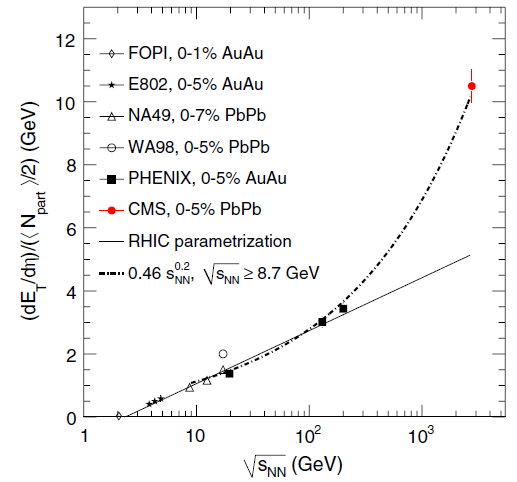
\includegraphics[width=.65\textwidth]{dEtdEta}
          \caption{Comparison of $\frac{dE_{T}}{d\eta}$ as a function of 
            collision energy, $\sqrt{s_{NN}}$, normalized by the number 
            participating nucleons, $N_{p}$, to account for the difference in 
            the ion species collided at the various different experiments.}
          \label{fig:dEtdEta}
        \end{figure}
  
      Direct photons, thermal photon created in the QGP, have been measured 
        at RHIC by PHENIX \cite{phenixPhoton2010} and at the LHC by ALICE 
        \cite{photonALICE} through the measurements of electron-positron pairs.
      Each experiment measured the inclusive \pt{} spectrum from 
        electron-positron pairs, all pairs from the sample are taken without
        regard to the creation mechanism.
      The PHENIX measurement was taken from pp collisions and top 20\% most 
        energetic AuAu collisions, collisions with a centrality of 0-20\%. 
      The ALICE measurement analyzed the 0-40\% centrality, 40\%-80\% centrality
        PbPb collisions, and pp collisions. 
      In both measurements, the contribution to the inclusive spectrum was sorted 
        into a direct component and a component from background, primary decays
        from hadrons such as pions and eta. 
      In the PHENIX measurement this was done by preforming a fit to the mass 
        distribution of the electron-positron pair for each \pt{}.
      For the ALICE measurement, the double ratio between the inclusive photons 
        to pions over the ratio between photons from hadron decays and pions was
        measured to estimate the direct contribution. 
      The inclusive photon \pt{} were then rescaled by the direct photon 
        fractions to produce a direct photon spectrum.
      The slope of an exponential fit to the low \pt{} portion the direct photon 
        spectrum is used to measure the temperature.
      \begin{figure}[!Hhbt]
        \centering
        $ \begin{array}{c c}
          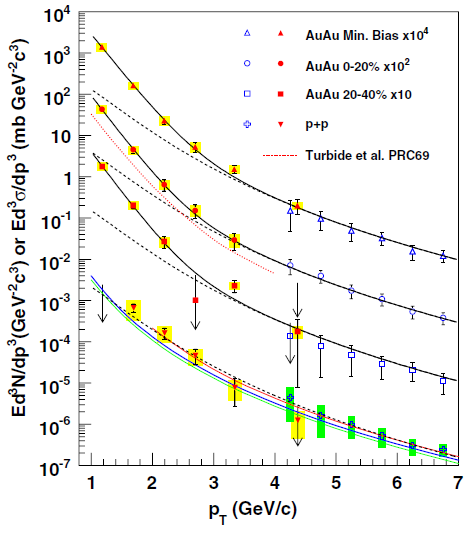
\includegraphics[width=.4\textwidth]{phenixDirectPhoton} &
          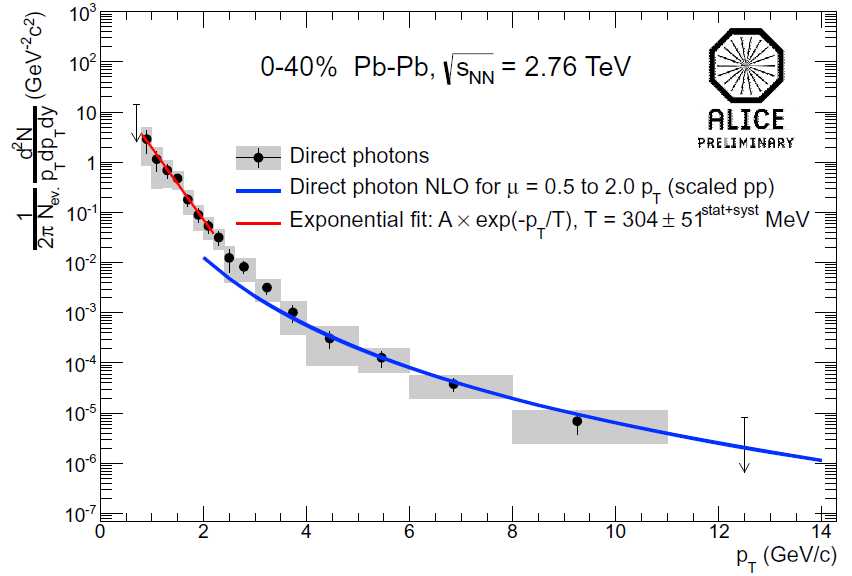
\includegraphics[width=.55\textwidth]{aliceDirectPhoton}
        \end{array} $
        \caption{Direct photon invariant yield as a function of \pt{} from 
          PHENIX \cite{phenixPhoton2010} (left) and ALICE \cite{photonALICE} 
          (right)}
        \label{fig:directPhotonPt}
      \end{figure}
  
      The direct photon through measurement of the temperature offers a clear 
        way of establishing whether the critical temperature for deconfinement
        was achieved. 
      The direct photon \pt{} spectra in Fig.~\ref{fig:directPhotonPt} show a 
        clear enhancement at low \pt{} compared to the rescaling to the pp 
        spectra that fits the high \pt{} part of the spectrum, indicating a 
        clear deviation for pp collisions.
      The low \pt{} photons therefore primarily come directly from the thermal 
        activity of the QGP.
      The thermal spectrum of the QGP is therefor imprinted on this part of the 
        spectrum.
      The exponential fits to the spectra provide this temperature. 
      The temperature from PHENIX was measured to be 221 $\pm$ 21 MeV and 
        304 $\pm$ 51 MeV from ALICE, both well above the critical temperature
        estimated from lattice QCD of $\sim$ 170 MeV.
  
      The combination of the energy density and temperture measurements
        create a consistent picture, both RHIC and the LHC have created a 
        deconfined state, and due the higher collision energies at the LHC the 
        the medium gets hotter. 

    \subsection{Elliptic flow and viscosity in the QGP}
      Prior to the RHIC, the QGP was thought to be a gas of quarks and gluons.
      At RHIC, elliptic flow, $v2$, was measured by PHOBOS \cite{phobosFlow} and the other 
        RHIC experiments showed that the medium appeared to obey hydrodynamic equations and 
        flows like a fluid.
      This same signal was also measured by CMS\cite{cmsFlow} at the LHC. 

      Elliptic flow, $v^{2}$, is second order coefficient of the Fourier 
        expansion of the azimuthal distribution of measured tracks.
      This expansion has the form,
      \begin{equation}
        1+\sum^{\infty}_{n=1}2v_{n}\mathrm{cos}\left[n\left(\phi-\Psi\right)\right],
        \label{eg:v2Expand}
      \end{equation}
        where $v_{n}$ is the $n$th coefficient of the Fourier expansion, $\phi$
        is the azimuthal angle, and $\Psi$ is the event-plane angle.
      The event-plane angle accounts for the random orientation of the 
        nuclei event by event and is correlated with the reaction-plane
        , $\Psi_{R}$ (see Fig.~\ref{fig:elipSchem}).
        
      \begin{figure}[!Hhbt]
        \centering
        $ \begin{array}{cc}
        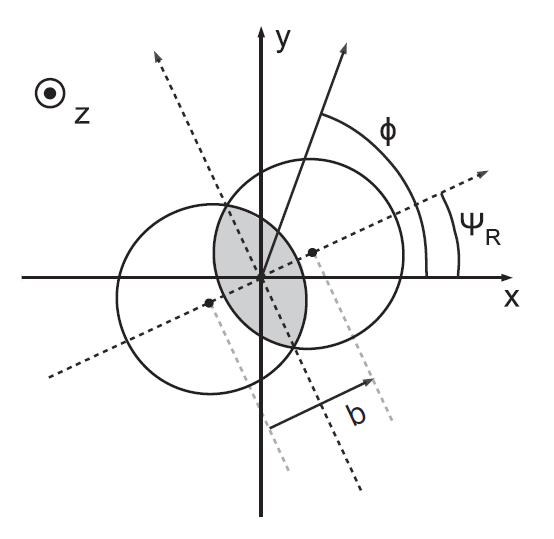
\includegraphics[width=.45\textwidth]{elipFlowSchemCMSGrey} &
        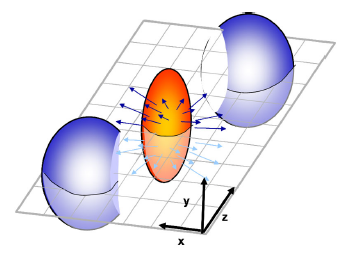
\includegraphics[width=.45\textwidth]{elipFlowSchem}
        \end{array} $
        \caption{Schematic of the initial nuclear overlap and elliptic flow.}
        \label{fig:elipSchem}
      \end{figure}
  
      The $v^{2}$ signal is believed to arise from the pressure gradients 
        created by initial elliptical shape of overlap region of the 
        two colliding nuclei. 
      The pressure gradient is higher along the shorter axis compared to 
        the longer axis of the ellipsoid in Fig~\ref{fig:elipSchem}.
      This difference in pressure gradient will create a flow of the QGP 
        medium in the direction of the shorter axis. 
      The flow in turn creates a preferred for the particles in $\phi$, which
        produces the measured anisotropic distribution of tracks. 

      The extent to which the initial shape of the overlap translates to flow
        in the medium is controlled by the viscosity of the medium. 
      A viscous fluid will tend to smooth out anisotropies and results in 
        a smaller flow signal for the same overlap configuration of the initial
        nuclei. 
      The ratio between the measured $v^{2}$ signal and the initial 
        eccentricity, $\epsilon$, based on the given centrality can is sensitive
        to the viscosity of the medium. 

      \begin{figure}[!Hhbt]
        \centering
        $ \begin{array}{cc}
          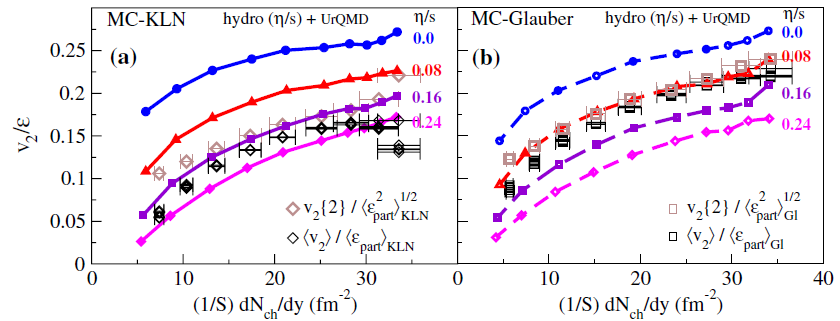
\includegraphics[width=.75\textwidth]{etaOvSinit} \\
          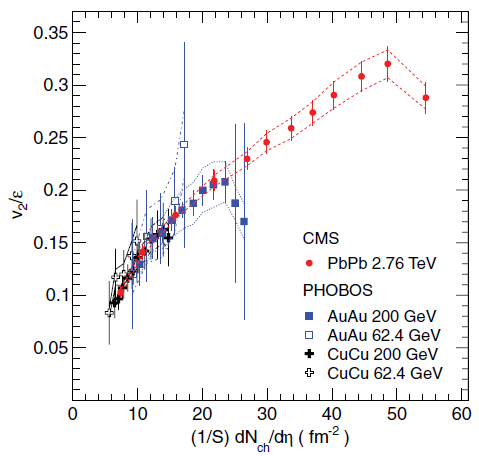
\includegraphics[width=.75\textwidth]{elipFlowCMS}
        \end{array} $
        \caption{$v^{2}/\epsilon$  as a function of $1/S \frac{dN_{ch}}{dy}$
          for different different values of $\eta/s$ for KLN initial state 
          (left) and Glauber initial state (center) compared to STAR (overlaid)
          and CMS and PHOBOS data (right).}
        \label{fig:elipFlow}
      \end{figure}

      In Fig.~\ref{fig:elipFlow} $v^{2}/\epsilon$ is as a function of number 
        of charged particle, $N_{ch}$, pre pseudorapidity, $\eta$, per area of 
        overlap between the colliding nuclei, $S$ \cite{etaOvSinit}. 
      The model calculation was performed for four values of the ratio of the 
        shear viscosity over entropy density, $\frac{\eta }{s}$, 0.0, 0.08, 
        0.16, and 0.24.
      The $\eta/s$ value which gives the best agreement with STAR data\cite{starFlow}
        overlaid on the theory calculations and that CMS and PHOBOS data to
        the right depends strong initial state model.
      This strong depends on the initial state is one of the primary reason
        more studies are needed of the initial state. 
      
    \subsection{Recent results from HI control measurements}
